\documentclass{article}\usepackage[]{graphicx}\usepackage[]{color}
%% maxwidth is the original width if it is less than linewidth
%% otherwise use linewidth (to make sure the graphics do not exceed the margin)
\makeatletter
\def\maxwidth{ %
  \ifdim\Gin@nat@width>\linewidth
    \linewidth
  \else
    \Gin@nat@width
  \fi
}
\makeatother

\definecolor{fgcolor}{rgb}{0.345, 0.345, 0.345}
\newcommand{\hlnum}[1]{\textcolor[rgb]{0.686,0.059,0.569}{#1}}%
\newcommand{\hlstr}[1]{\textcolor[rgb]{0.192,0.494,0.8}{#1}}%
\newcommand{\hlcom}[1]{\textcolor[rgb]{0.678,0.584,0.686}{\textit{#1}}}%
\newcommand{\hlopt}[1]{\textcolor[rgb]{0,0,0}{#1}}%
\newcommand{\hlstd}[1]{\textcolor[rgb]{0.345,0.345,0.345}{#1}}%
\newcommand{\hlkwa}[1]{\textcolor[rgb]{0.161,0.373,0.58}{\textbf{#1}}}%
\newcommand{\hlkwb}[1]{\textcolor[rgb]{0.69,0.353,0.396}{#1}}%
\newcommand{\hlkwc}[1]{\textcolor[rgb]{0.333,0.667,0.333}{#1}}%
\newcommand{\hlkwd}[1]{\textcolor[rgb]{0.737,0.353,0.396}{\textbf{#1}}}%
\let\hlipl\hlkwb

\usepackage{framed}
\makeatletter
\newenvironment{kframe}{%
 \def\at@end@of@kframe{}%
 \ifinner\ifhmode%
  \def\at@end@of@kframe{\end{minipage}}%
  \begin{minipage}{\columnwidth}%
 \fi\fi%
 \def\FrameCommand##1{\hskip\@totalleftmargin \hskip-\fboxsep
 \colorbox{shadecolor}{##1}\hskip-\fboxsep
     % There is no \\@totalrightmargin, so:
     \hskip-\linewidth \hskip-\@totalleftmargin \hskip\columnwidth}%
 \MakeFramed {\advance\hsize-\width
   \@totalleftmargin\z@ \linewidth\hsize
   \@setminipage}}%
 {\par\unskip\endMakeFramed%
 \at@end@of@kframe}
\makeatother

\definecolor{shadecolor}{rgb}{.97, .97, .97}
\definecolor{messagecolor}{rgb}{0, 0, 0}
\definecolor{warningcolor}{rgb}{1, 0, 1}
\definecolor{errorcolor}{rgb}{1, 0, 0}
\newenvironment{knitrout}{}{} % an empty environment to be redefined in TeX

\usepackage{alltt}
\usepackage{amsmath, amsthm, amsfonts}
\title{Assignment 1}
\IfFileExists{upquote.sty}{\usepackage{upquote}}{}
\begin{document}
\maketitle

{\color{red}For grader: Please comment in red. Either ``Everything is correct!'' or commenting to help your fellow classmate out if you think anything can be improved. If you use Markdown, bolded text is fine.

The cross-grading deadline is the end of the same week as the homework. We TAs will review your cross-grading and assign final numerical grade.}




\section*{Corruption and Wealth (3 points)}

\subsection*{Regression of corruption on GDP per capita}

\begin{knitrout}
\definecolor{shadecolor}{rgb}{0.969, 0.969, 0.969}\color{fgcolor}\begin{kframe}
\begin{alltt}
\hlstd{df_corruption} \hlkwb{<-} \hlstd{haven}\hlopt{::}\hlkwd{read_dta}\hlstd{(}\hlstr{"corruption.dta"}\hlstd{)}
\end{alltt}
\end{kframe}
\end{knitrout}

Running regression using OLS

\begin{kframe}
\begin{alltt}
\hlstd{m1} \hlkwb{<-} \hlkwd{lm}\hlstd{(ti_cpi} \hlopt{~} \hlstd{undp_gdp,} \hlkwc{data} \hlstd{= df_corruption)}
\hlkwd{stargazer}\hlstd{(m1)}
\end{alltt}
\end{kframe}
% Table created by stargazer v.5.2 by Marek Hlavac, Harvard University. E-mail: hlavac at fas.harvard.edu
% Date and time: Thu, Feb 22, 2018 - 11:10:54 AM
\begin{table}[!htbp] \centering 
  \caption{} 
  \label{} 
\begin{tabular}{@{\extracolsep{5pt}}lc} 
\\[-1.8ex]\hline 
\hline \\[-1.8ex] 
 & \multicolumn{1}{c}{\textit{Dependent variable:}} \\ 
\cline{2-2} 
\\[-1.8ex] & ti\_cpi \\ 
\hline \\[-1.8ex] 
 undp\_gdp & 0.0002$^{***}$ \\ 
  & (0.00001) \\ 
  & \\ 
 Constant & 2.502$^{***}$ \\ 
  & (0.124) \\ 
  & \\ 
\hline \\[-1.8ex] 
Observations & 170 \\ 
R$^{2}$ & 0.673 \\ 
Adjusted R$^{2}$ & 0.671 \\ 
Residual Std. Error & 1.207 (df = 168) \\ 
F Statistic & 346.398$^{***}$ (df = 1; 168) \\ 
\hline 
\hline \\[-1.8ex] 
\textit{Note:}  & \multicolumn{1}{r}{$^{*}$p$<$0.1; $^{**}$p$<$0.05; $^{***}$p$<$0.01} \\ 
\end{tabular} 
\end{table} 


Running regression using MLE

Note that the likelihood function is

\begin{align}
Y &\sim N(X\beta, \sigma^2) \\
LL &= \sum_i \log N(X\beta, \sigma^2)
\end{align}

\begin{knitrout}
\definecolor{shadecolor}{rgb}{0.969, 0.969, 0.969}\color{fgcolor}\begin{kframe}
\begin{alltt}
\hlstd{X} \hlkwb{<-} \hlkwd{cbind}\hlstd{(}\hlnum{1}\hlstd{, df_corruption}\hlopt{$}\hlstd{undp_gdp)}
\hlstd{y} \hlkwb{<-} \hlstd{df_corruption}\hlopt{$}\hlstd{ti_cpi}
\hlstd{N} \hlkwb{<-} \hlkwd{length}\hlstd{(y)}
\hlcom{#' The loglikelihood is a function of beta and sigma2. This is a direct}
\hlcom{#' implementation of the formula on slide MLE week 3, p 30}
\hlcom{#' @param params is a vector of length 3, }
\hlcom{#' the 1st element is beta for the intercept, }
\hlcom{#' the 2nd element is beta for GDP per capita,}
\hlcom{#' the 3rd element is sigma2}
\hlstd{negative_log_likelihood} \hlkwb{<-} \hlkwa{function}\hlstd{(}\hlkwc{params}\hlstd{) \{}
  \hlstd{beta} \hlkwb{<-} \hlkwd{c}\hlstd{(params[}\hlnum{1}\hlstd{], params[}\hlnum{2}\hlstd{])}
  \hlstd{sigma2} \hlkwb{<-} \hlstd{params[}\hlnum{3}\hlstd{]}
  \hlkwd{return}\hlstd{(N} \hlopt{/} \hlnum{2} \hlopt{*} \hlkwd{log}\hlstd{(sigma2)} \hlopt{+}
         \hlnum{1} \hlopt{/} \hlstd{(}\hlnum{2} \hlopt{*} \hlstd{sigma2)} \hlopt{*} \hlkwd{t}\hlstd{(y} \hlopt{-} \hlstd{X} \hlopt \hlstd{beta)} \hlopt \hlstd{(y} \hlopt{-} \hlstd{X} \hlopt \hlstd{beta))}
\hlstd{\}}

\hlcom{# MLE estimate}
\hlstd{m2} \hlkwb{<-} \hlkwd{optim}\hlstd{(}\hlkwc{par} \hlstd{=} \hlkwd{c}\hlstd{(}\hlnum{0}\hlstd{,} \hlnum{0}\hlstd{,} \hlnum{1}\hlstd{),} \hlkwc{fn} \hlstd{= negative_log_likelihood)}\hlopt{$}\hlstd{par}
\hlkwd{names}\hlstd{(m2)} \hlkwb{<-} \hlkwd{c}\hlstd{(}\hlstr{"beta0"}\hlstd{,} \hlstr{"beta1"}\hlstd{,} \hlstr{"sigma2"}\hlstd{)}
\hlkwd{print}\hlstd{(m2)}
\end{alltt}
\begin{verbatim}
##        beta0        beta1       sigma2 
## 2.5027995972 0.0001729247 1.4381806067
\end{verbatim}
\end{kframe}
\end{knitrout}

We see that the MLE for $\beta$ from \verb`optim` result are 2.5027996, \ensuremath{1.7292473\times 10^{-4}}, exactly as the OLS result above.

The intercept means that when a country has a GDP per capita of 0, its predicted corruption level (in terms of CPI score) is 2.503.

The coefficient for GDP per capita means that an increase of USD 1000 in GDP per capita is associated with a change of 0.173 in corruption level (in terms of CPI score).

\subsection*{Interpret the substantive relevance}

\begin{knitrout}
\definecolor{shadecolor}{rgb}{0.969, 0.969, 0.969}\color{fgcolor}\begin{kframe}
\begin{alltt}
\hlstd{new_data} \hlkwb{<-} \hlkwd{data.frame}\hlstd{(}\hlkwc{undp_gdp} \hlstd{=} \hlkwd{quantile}\hlstd{(df_corruption}\hlopt{$}\hlstd{undp_gdp,}
                                           \hlkwd{c}\hlstd{(}\hlnum{0.25}\hlstd{,} \hlnum{0.75}\hlstd{)))}
\hlstd{pred_m1} \hlkwb{<-} \hlkwd{predict}\hlstd{(m1,} \hlkwc{newdata} \hlstd{= new_data)}
\hlkwd{print}\hlstd{(pred_m1)}
\end{alltt}
\begin{verbatim}
##      25%      75% 
## 2.843991 4.381464
\end{verbatim}
\end{kframe}
\end{knitrout}


The level of corruption in countries with GDP per capita that corresponds to the 25th percentile is 2.844 and a country with GDP per capita in the 75th percentile is 4.381.

\section*{Maximum Likelihood I (3 points)}

\subsection*{1.} Logit and probit coefficients always differ because the error terms in the two models are normalized to have a different scale.

More specifically, recall that both probit and logit are derived from the following random utility model:

\begin{align}
U_i^* &= \beta_0^* + \beta_1^* X + \epsilon^*
\end{align}

where $\epsilon^*$ is the unobserved component of the utility. Call the standard deviation of this unobserved component $\sigma$ (which is unknown, because we don't observe $\epsilon^*$). 

In probit, we want to normalize so that the error term is normally distributed with a standard deviation of 1. We do this by dividing everything by $\sigma$:

\begin{align}
U_i &= \frac{\beta_0^*}{\sigma} + \frac{\beta_1^*}{\sigma} X + \frac{\epsilon^*}{\sigma} \\
\end{align}

In logit, we want to normalize so that the error term is follows standard Gumbel distribution, with a standard deviation of $\sqrt{\pi^2 / 6} \sim \sqrt{1.6}$. We do this by dividing everything by $\frac{\sigma}{\sqrt{1.6}}$

\begin{align}
U_i &= \frac{\sqrt{1.6}\beta_0^*}{\sigma} + \frac{\sqrt{1.6}\beta_1^*}{\sigma} X + \frac{\sqrt{1.6}\epsilon^*}{\sigma} \\
\end{align}

As you can see, the coefficient we get from probit is $\frac{\beta_1^*}{\sigma}$, while the coefficient we get from logit is $\frac{\sqrt{1.6}\beta_1^*}{\sigma}$. So the logit's coefficient is always $\sqrt{1.6}$ times larger than probit's.

\subsection*{2.} Predicted values from a binary model are either 0 or 1. The expected value is the expectation of the predicted value, which for binary model is the probability that the outcome is 1.

\subsection*{3.} A binomial distribution is usually used to model the number of successes in N trials. Here we can consider each student as a trial, and a pass as a success. 

Define $y$ as the number of passes, we have:

\begin{align}
y &\sim Binom(13, \theta) \\
lik &= {13 \choose y} \theta^y (1 - \theta)^{n - y}
\end{align}

\section*{Maximum Likelihood II (4 points)}

\begin{kframe}
\begin{alltt}
\hlstd{df_turnout} \hlkwb{<-} \hlstd{haven}\hlopt{::}\hlkwd{read_dta}\hlstd{(}\hlstr{"turnout.dta"}\hlstd{)}
\hlstd{m_turnout} \hlkwb{<-} \hlkwd{glm}\hlstd{(voted} \hlopt{~} \hlstd{informed} \hlopt{+} \hlstd{age} \hlopt{+} \hlstd{edu} \hlopt{+} \hlstd{female,} \hlkwc{data} \hlstd{= df_turnout,}
                 \hlkwc{family} \hlstd{= binomial)}
\hlstd{summary_turnout} \hlkwb{<-} \hlkwd{summary}\hlstd{(m_turnout)}
\hlkwd{stargazer}\hlstd{(m_turnout)}
\end{alltt}
\end{kframe}
% Table created by stargazer v.5.2 by Marek Hlavac, Harvard University. E-mail: hlavac at fas.harvard.edu
% Date and time: Thu, Feb 22, 2018 - 11:10:59 AM
\begin{table}[!htbp] \centering 
  \caption{} 
  \label{} 
\begin{tabular}{@{\extracolsep{5pt}}lc} 
\\[-1.8ex]\hline 
\hline \\[-1.8ex] 
 & \multicolumn{1}{c}{\textit{Dependent variable:}} \\ 
\cline{2-2} 
\\[-1.8ex] & voted \\ 
\hline \\[-1.8ex] 
 informed & 0.522$^{***}$ \\ 
  & (0.103) \\ 
  & \\ 
 age & 0.032$^{***}$ \\ 
  & (0.005) \\ 
  & \\ 
 edu & 0.343$^{***}$ \\ 
  & (0.088) \\ 
  & \\ 
 female & 0.427$^{***}$ \\ 
  & (0.162) \\ 
  & \\ 
 Constant & $-$2.495$^{***}$ \\ 
  & (0.428) \\ 
  & \\ 
\hline \\[-1.8ex] 
Observations & 1,078 \\ 
Log Likelihood & $-$514.638 \\ 
Akaike Inf. Crit. & 1,039.276 \\ 
\hline 
\hline \\[-1.8ex] 
\textit{Note:}  & \multicolumn{1}{r}{$^{*}$p$<$0.1; $^{**}$p$<$0.05; $^{***}$p$<$0.01} \\ 
\end{tabular} 
\end{table} 


\subsection*{1.} 

The $\beta$ for \verb`female` is 0.427, meaning that the odd of voting is $\exp(\beta) = $ 1.533 times larger for female.

\subsection*{2.}

Predicted probability of turnout for woman, age = 25, edu = 3, and average political information is

\begin{knitrout}
\definecolor{shadecolor}{rgb}{0.969, 0.969, 0.969}\color{fgcolor}\begin{kframe}
\begin{alltt}
\hlkwd{predict}\hlstd{(m_turnout,}
        \hlkwc{newdata} \hlstd{=} \hlkwd{data.frame}\hlstd{(}\hlkwc{female} \hlstd{=} \hlnum{1}\hlstd{,} \hlkwc{age} \hlstd{=} \hlnum{25}\hlstd{,} \hlkwc{edu} \hlstd{=} \hlnum{3}\hlstd{,}
                             \hlkwc{informed} \hlstd{=} \hlkwd{mean}\hlstd{(df_turnout}\hlopt{$}\hlstd{informed)),}
        \hlkwc{type} \hlstd{=} \hlstr{"response"}\hlstd{)}
\end{alltt}
\begin{verbatim}
##         1 
## 0.8065287
\end{verbatim}
\end{kframe}
\end{knitrout}

\subsection*{3.}

To show the effect of political information at low [0] and high [3] education level, we calculate the probability of voting. We use simulation to demonstrate uncertainty

\begin{knitrout}
\definecolor{shadecolor}{rgb}{0.969, 0.969, 0.969}\color{fgcolor}\begin{kframe}
\begin{alltt}
\hlstd{S} \hlkwb{<-} \hlnum{1000} \hlcom{# Number of simulations}
\hlstd{beta_hat} \hlkwb{<-} \hlkwd{coef}\hlstd{(m_turnout)}
\hlstd{V_beta_hat} \hlkwb{<-} \hlstd{summary_turnout}\hlopt{$}\hlstd{cov.unscaled}

\hlcom{# Draw an estimate from N(beta_hat, V_beta_hat)}
\hlstd{beta} \hlkwb{<-} \hlstd{mvtnorm}\hlopt{::}\hlkwd{rmvnorm}\hlstd{(S,} \hlkwc{mean} \hlstd{= beta_hat,} \hlkwc{sigma} \hlstd{= V_beta_hat)}
\end{alltt}
\end{kframe}
\end{knitrout}

\begin{knitrout}
\definecolor{shadecolor}{rgb}{0.969, 0.969, 0.969}\color{fgcolor}\begin{kframe}
\begin{alltt}
\hlcom{# Set other values}
\hlstd{X_edulow} \hlkwb{<-} \hlkwd{data.frame}\hlstd{(}\hlkwc{intercept} \hlstd{=} \hlnum{1}\hlstd{,}
                       \hlkwc{informed} \hlstd{=} \hlnum{1}\hlopt{:}\hlnum{4}\hlstd{,}
                       \hlkwc{age} \hlstd{=} \hlkwd{mean}\hlstd{(df_turnout}\hlopt{$}\hlstd{age),}
                       \hlkwc{edu} \hlstd{=} \hlnum{0}\hlstd{,}
                       \hlkwc{female} \hlstd{=} \hlnum{0}\hlstd{)} \hlopt \hlkwd{as.matrix}\hlstd{()}
\hlstd{XB} \hlkwb{<-} \hlstd{beta} \hlopt \hlkwd{t}\hlstd{(X_edulow)}
\hlstd{predicted_probs} \hlkwb{<-} \hlkwd{exp}\hlstd{(XB)} \hlopt{/} \hlstd{(}\hlnum{1} \hlopt{+} \hlkwd{exp}\hlstd{(XB))}
\hlstd{dat_edulow} \hlkwb{<-} \hlkwd{as.data.frame}\hlstd{(predicted_probs)} \hlopt
  \hlstd{tidyr}\hlopt{::}\hlkwd{gather}\hlstd{(}\hlkwc{key} \hlstd{=} \hlstr{"informed"}\hlstd{,} \hlkwc{value} \hlstd{=} \hlstr{"predicted_prob"}\hlstd{)} \hlopt
  \hlkwd{mutate}\hlstd{(}\hlkwc{informed} \hlstd{=} \hlkwd{recode}\hlstd{(informed,} \hlstr{"V1"} \hlstd{=} \hlnum{1}\hlstd{,} \hlstr{"V2"} \hlstd{=} \hlnum{2}\hlstd{,} \hlstr{"V3"} \hlstd{=} \hlnum{3}\hlstd{,} \hlstr{"V4"} \hlstd{=} \hlnum{4}\hlstd{),}
         \hlkwc{edu} \hlstd{=} \hlstr{"low"}\hlstd{)}

\hlcom{# Set values and calculate predicted_probs}
\hlstd{X_eduhigh} \hlkwb{<-} \hlkwd{data.frame}\hlstd{(}\hlkwc{intercept} \hlstd{=} \hlnum{1}\hlstd{,}
                       \hlkwc{informed} \hlstd{=} \hlnum{1}\hlopt{:}\hlnum{4}\hlstd{,}
                       \hlkwc{age} \hlstd{=} \hlkwd{mean}\hlstd{(df_turnout}\hlopt{$}\hlstd{age),}
                       \hlkwc{edu} \hlstd{=} \hlnum{3}\hlstd{,}
                       \hlkwc{female} \hlstd{=} \hlnum{0}\hlstd{)} \hlopt \hlkwd{as.matrix}\hlstd{()}
\hlstd{XB} \hlkwb{<-} \hlstd{beta} \hlopt \hlkwd{t}\hlstd{(X_eduhigh)}
\hlstd{predicted_probs} \hlkwb{<-} \hlkwd{exp}\hlstd{(XB)} \hlopt{/} \hlstd{(}\hlnum{1} \hlopt{+} \hlkwd{exp}\hlstd{(XB))}
\hlstd{dat_eduhigh} \hlkwb{<-} \hlkwd{as.data.frame}\hlstd{(predicted_probs)} \hlopt
  \hlstd{tidyr}\hlopt{::}\hlkwd{gather}\hlstd{(}\hlkwc{key} \hlstd{=} \hlstr{"informed"}\hlstd{,} \hlkwc{value} \hlstd{=} \hlstr{"predicted_prob"}\hlstd{)} \hlopt
  \hlkwd{mutate}\hlstd{(}\hlkwc{informed} \hlstd{=} \hlkwd{recode}\hlstd{(informed,} \hlstr{"V1"} \hlstd{=} \hlnum{1}\hlstd{,} \hlstr{"V2"} \hlstd{=} \hlnum{2}\hlstd{,} \hlstr{"V3"} \hlstd{=} \hlnum{3}\hlstd{,} \hlstr{"V4"} \hlstd{=} \hlnum{4}\hlstd{),}
         \hlkwc{edu} \hlstd{=} \hlstr{"high"}\hlstd{)}


\hlstd{dat} \hlkwb{<-} \hlkwd{bind_rows}\hlstd{(}\hlkwd{list}\hlstd{(dat_edulow, dat_eduhigh))}
\end{alltt}
\end{kframe}
\end{knitrout}

Below we plot the predicted probability of voting across levels of political information. For respondents with low education, the probability of voting increases from 0.4 $\pm$ 0.1 to 0.7 $\pm$ 0.08 as the level of political information increases from 1 to 4. For respondents with high education, the probability of voting increases from 0.6 $\pm$ 0.1 to 0.9 $\pm$ 0.03 as the level of political information increases from 1 to 4. (The error bars reflect the 95\% confidence interval. The uncertainty is highest for respondents where \verb`informed = 1` because we have the least amount of data for them.)

Overall, the level of political information has a positive effect on the probability of voting. The size of the effect is also consistent across both high and low education respondents.

\begin{knitrout}
\definecolor{shadecolor}{rgb}{0.969, 0.969, 0.969}\color{fgcolor}\begin{kframe}
\begin{alltt}
\hlkwd{ggplot}\hlstd{(}\hlkwc{data} \hlstd{= dat,} \hlkwd{aes}\hlstd{(}\hlkwc{x} \hlstd{= informed,} \hlkwc{y} \hlstd{= predicted_prob,} \hlkwc{color} \hlstd{= edu))} \hlopt{+}
  \hlkwd{stat_summary}\hlstd{(}\hlkwc{fun.y} \hlstd{= mean,}
               \hlkwc{fun.ymin} \hlstd{=} \hlkwa{function}\hlstd{(}\hlkwc{x}\hlstd{)} \hlkwd{mean}\hlstd{(x)} \hlopt{-} \hlnum{1.96} \hlopt{*} \hlkwd{sd}\hlstd{(x),}
               \hlkwc{fun.ymax} \hlstd{=} \hlkwa{function}\hlstd{(}\hlkwc{x}\hlstd{)} \hlkwd{mean}\hlstd{(x)} \hlopt{+} \hlnum{1.96} \hlopt{*} \hlkwd{sd}\hlstd{(x),}
               \hlkwc{geom} \hlstd{=} \hlstr{"pointrange"}\hlstd{)} \hlopt{+}
  \hlkwd{stat_summary}\hlstd{(}\hlkwc{fun.y} \hlstd{= mean,} \hlkwc{geom} \hlstd{=} \hlstr{"line"}\hlstd{)} \hlopt{+}
  \hlkwd{labs}\hlstd{(}\hlkwc{x} \hlstd{=} \hlstr{"Level of Political Information"}\hlstd{,} \hlkwc{y} \hlstd{=} \hlstr{"Predicted Prob of Voting"}\hlstd{)}
\end{alltt}
\end{kframe}
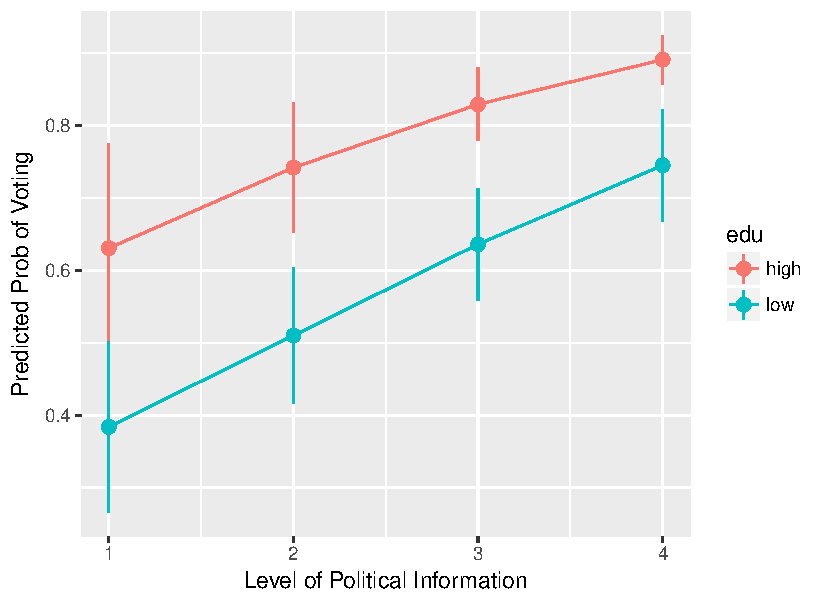
\includegraphics[width=\maxwidth]{figure/unnamed-chunk-10-1} 

\end{knitrout}


\end{document}
